\subsubsection{Tyk}
\label{soa:tecnologias:tyk}

Tyk es un API Gateway liviano y plataforma de administración, todo en un mismo producto, que permite controlar quien tiene acceso a la API, cuando y como.  Escrito en Go, sencillo de configurar, sus únicas dependencias son Redis y MongoDB (v2.6 o superior, requerido para el almacenamiento de los datos de acceso, opcional)

El API Gateway de Tyk se implementa delante de nuestras \glspl{acro:api} para gestionar la autorización, control de acceso y limitación de acceso (\eng{rate limiting}) a nuetros servicios.  De esta manera permite concentranos en el desarrollo de servicios para nuestras \glspl{acro:api}, en lugar de implementar herramientas para la administración de la infraestrucutra, simplemente se desarrollo el servicio, el cual puede ser integrado fácilmente al API Gateway.

Tyk posee un portal para desarrolladores que permite analizar quien y como utilizan nuestras \glspl{acro:api}, limitar el acceso a los servicios (\eng{rate limiting}), utlización de \eng{caching}, generar o rebocar una \eng{Key}, entro otras características.  Todo esto de manera muy sencilla y centralizada, evitando trasladar parte de esta funcionalidad a las \glspl{acro:api}.

\paragraph{Licencia}

Tyk se encuentra publicado bajo licencia Mozilla Public License Version 2.0\footnote{La misma puede ser consultada accediendo a \url{https://www.mozilla.org/en-US/MPL/2.0}}.

\paragraph{Características principales}

A continuación presentamos un breve listado de las características principales que Tyk ofrece actualmente:

\begin{itemize}
  \item RESTful API - posee una \gls{acro:api} RESTful, que permite configurar Tyk.
  \item Multiple access protocols - Tyk soporta múltiples métodos de acceso a la \gls{acro:api}: \eng{Token-based}, \eng{HMAC}, \eng{Basic Auth}, \eng{OAuth2}, \eng{JSON Web Token} y \eng{Keyless}. \\
  \url{https://tyk.io/v1.9/access-control/keyless} \\
  \url{https://tyk.io/v1.9/access-control/json-web-tokens} \\
  \url{https://tyk.io/v1.9/access-control/basic-auth} \\
  \url{https://tyk.io/v1.9/access-control/hmac} \\
  \item Rate Limiting - permite configurar fácilmente el \eng{rate limit} para cada \eng{API Key}, definiendo la cantidad de peticiones por segundo y el tiempo de expiración (1 hora, 6 horas, 12 horas, 24 horas, 1 semana, 1 mes o nunca expira). \\
  \url{https://tyk.io/v1.9/quotas-limits-security/access-control}
  \item Policies - permite crear políticas para aplicar \eng{quotas}, \eng{rate limit} y \eng{access rights} a un conjunto de \eng{Keys}. \\
  \url{https://tyk.io/v1.9/quotas-limits-security/limiting-access}
  \item Path by path permissions - permite configurar permisos de acceso para cada \eng{endpoint}, indicando el método.
  \item Key Expiry - permite controlar el tiempo de expiración de una \eng{Key}. \\
  \url{https://tyk.io/v1.9/rest-api/api-key-management}
  \item API Versioning - permite versionar la API de tres maneras diferentes:
  \begin{itemize}
    \item mediante una clave en el encabezado http, por ej. x-api-version
    \item por URL o parámetro en el Form
    \item por el primer elemento de una URL, ej. /v1/resource/id
  \end{itemize}
  \url{https://tyk.io/v1.9/api-management/api-versioning}
  \item Analyitcs logging - registro detallado de los accesos a las \glspl{acro:api}.
  \item Zero downtime restarts - las configuraciones de Tyk pueden realizarse dinámicamente, reiniciar los servicios sin que esto afecte los requerimientos activos.
  \item Web hooks - fácilmente se pueden integrar notificaciones y eventos que permitirán mejorar el monitoreo.
  \item IP White-listing - acceso autorizado solo a las direcciones IP indicadas
  \item Size Limits - permite limitar el tamañan de las peticiones que llegan a las \gls{acro:api}, evitando que los sevicios sean saturados por peticiones.
  \item Health checks - permite verificar el estado de los nodos.
  \item Mock APIs - permite crear \glspl{acro:api} de prueba.
  \item API Blueprint support - permite importar rápidamente una \gls{acro:api} en formato JSON.
  \item Swagger support - permite importar archivos que respeten \nameref{soa:tecnologias:openapi-spec} (anteriormente conocida como \eng{The Swagger specification}).
  \item Request and Response transformations - permite utilizar templates para transformar datos y agregar o quitar header \eng{on-the-fly}
  \item Caching - permite implementar una cache para las respuestas por \eng{endpoint} o globalmente, incrementando la velocidad de respuesta, al mismo tiempo que se disminuye la carga de las \gls{acro:api}. \\
  \url{https://tyk.io/v1.9/api-management/caching}
  \item API Documentation, el portal de Tyk soporta API Blueprint y Swagger.
  \item Virtual Endpoints, como AWS Lambda functions, permite correr fragmentos de JavaScript en los \eng{endpoints} para manejar interacciones complejas de servicios, tales como solicitud de procesamiento por lotes. \\
  \url{https://tyk.io/v1.9/api-management/virtual-endpoints}
  \item Focus on microservices, permite implementar el patrón \eng{circuit breaker}, hard timeouts y \eng{round-robin}, para balancear la carga en el acceso a los servicios. \\
  \url{https://tyk.io/v1.9/api-management/circuit-breakers} \\
  \url{https://tyk.io/v1.9/api-management/load-balancing}
  \item Uptime Awareness, Tyk activamente monitorea los \eng{endpoints} de las \glspl{acro:api} y notifica cuando alguno de estos se encuentra fuera de servicio. \\
  \url{https://tyk.io/v1.9/uptime-tests/uptime-tests}
\end{itemize}

\paragraph{Instalación y prueba}

A continuación se detallan los pasos necesarios para la instalación y ejecución de Tyk, basándonos en su documentación oficial \footnote{\url{https://tyk.io}}.

Tyk puede instalarse de varias maneras:

\begin{itemize}
  \item Instalación de Tyk en Ubuntu desde paquetes
  \item Instalación de Tyk en Redhat o CentOS usando paquetes RPM
  \item Instalación de Tyk desde una imagen Docker
\end{itemize}

En nuestro caso particular se optó por instalar Tyk en Ubuntu 14.04 desde paquetes, continuación desarrollaremos esta forma de instalación.

Pre-requisitos:

Asegurarse que el puerto 8080 esté abierto: este puerto es utlizado por el API Gateway
Asegurarse que el puerto 3000 esté abierto: este puerto es utlizado por el dashboard, quien provee la GUI y el portal para desarrolladores

\begin{listing}[H]
  \bashfile{src/03-capitulo-3/tecnologias/nodo-central/code/tyk/00-preparacion.sh}
  \caption{Preparación y arranque de Tyk}
  \label{soa:tecnologias:tyk:bash-preparacion}
\end{listing}


\paragraph{Integración con nuestro diseño}

Para el nuevo diseño de la arquitectura, se implementaría el API Gateway de Tyk como un nodo central, por donde se enrutarían todas las peticiones realizadas desde los diferentes clientes.  Detrás de Tyk tendremos replicadas N instancias de las \glspl{acro:api}, las cuales nos permiten escalar horizontalmente de forma sencilla, Tyk se encargará de realizar el balanceo de la carga a cualquiera de estas instancias replicadas.

La migración de la vieja nube a la nueva arquitectura, se iría realizando de manera progresiva, cambiando el viejo cliente por el nuevo, en cada aplicación.  De esta manera tendremos conviviendo al mismo tiempo, la vieja nube y la nueva arquitectura.

\begin{figure}[H]
  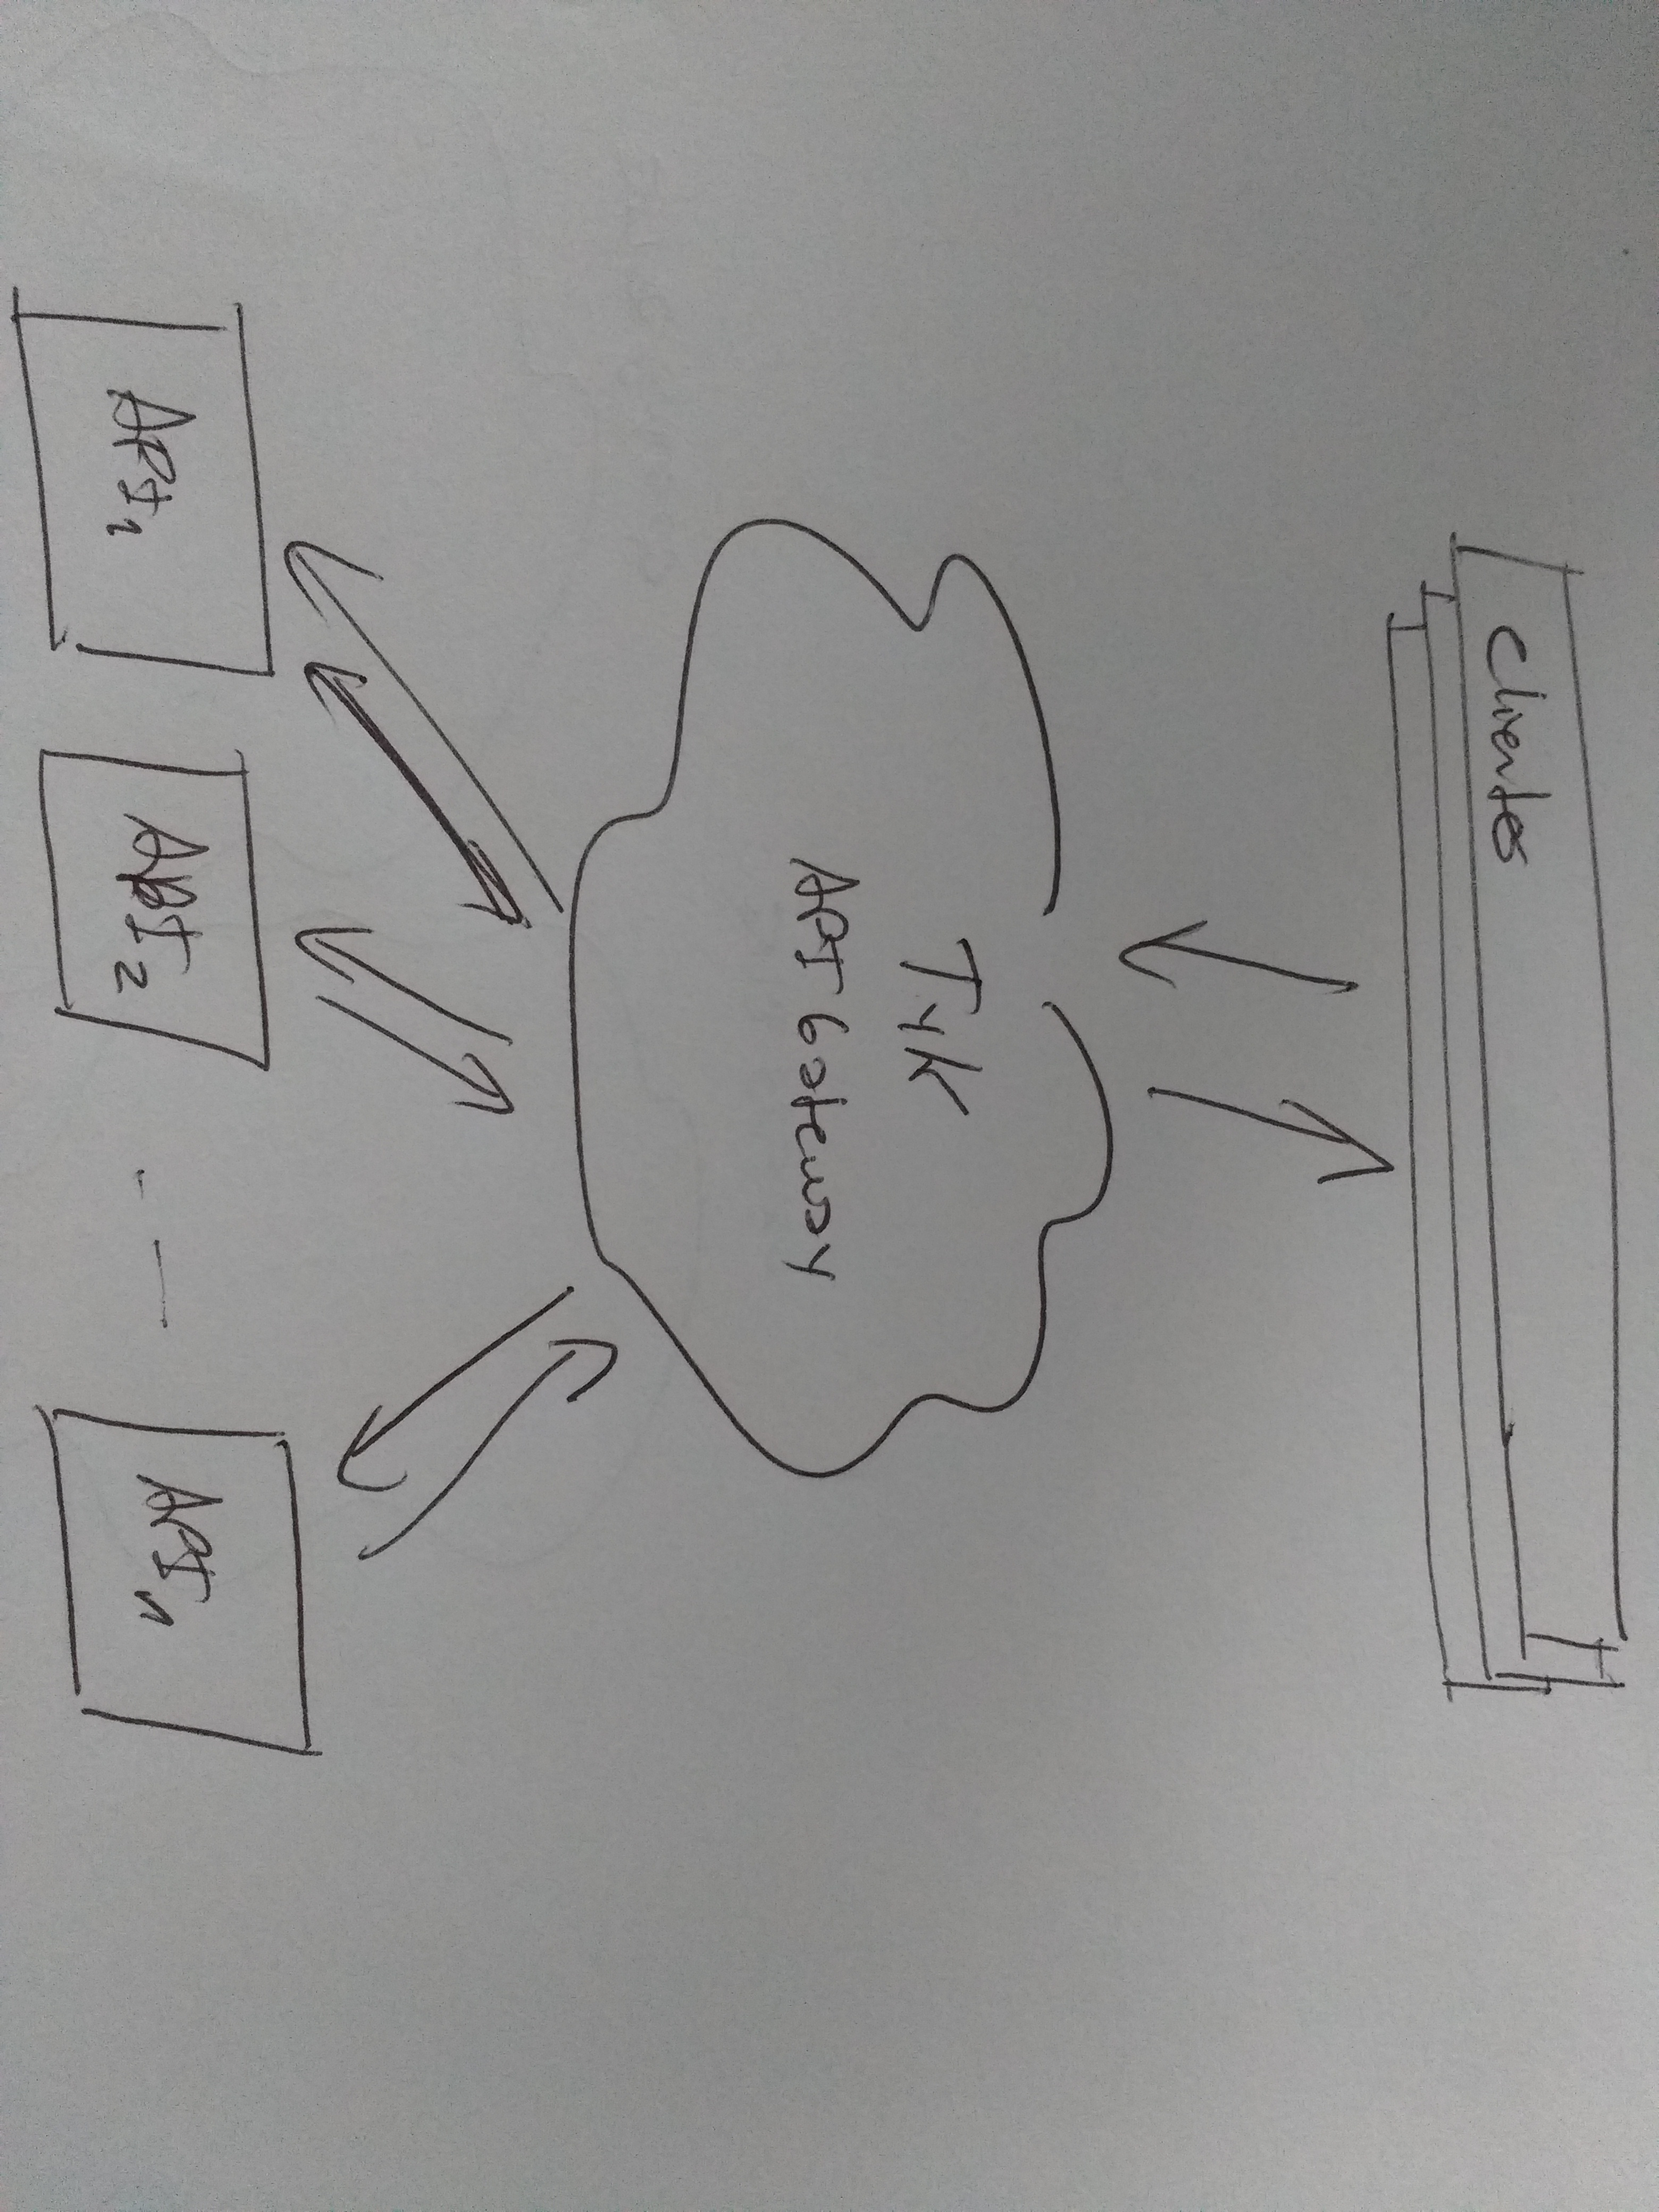
\includegraphics[width=\linewidth]{src/images/03-capitulo-3/tecnologias/tyk/tyk-arq.jpg}
  \caption{Esquema de integración de Tyk en nuestra propuesta}
  \label{fig:integracion-tyk-arquitectura}
\end{figure}
